\section{شرح پروژه}
- این که کلا دستگاه قراره چی کار کنه و اینا
\subsection{تغییرات نسبت به پروپوزال اولیه}
- این که قراره چند تا لوکیشن رو هندل کنیم
\section{طراحی و پیاده سازی}
- کلا iot builder و این داستانا رو یه ذره بگیم و نوع پروژه توی پرتئوس و اینا

در این پروژه ما با استفاده از 
\href{https://labcenter.s3.amazonaws.com/downloads/iotHelp.pdf}{iot-builder}
یک 
\subsection{شماتیک مدار}
شماتیک مدار را در شکل زیر مشاهده می‌کنید. در این مدار یک برد 
\lr{Arduino Yun}
که برای کاربرد‌های 
\lr{iot}
مناسب است و سه سنسور
\lr{LM35DZ}
تعبیه شده است که سنسور‌های دما هستند اما ما از آن‌ها به عنوان سنسور تشخیص گاز استفاده می‌کنیم. در پروپوزال ما سنسور‌های واقعی اندازه‌گیری گاز 
\lr{MQ-7}
و 
\lr{MQ-2}
و
\lr{MQ-135}
را استفاده کرده بودیم اما چون این سنسور‌ها در 
\lr{Proteus}
نبودند ما از سنسور‌های جایگزین اندازه‌گیری دما استفاده کردیم.
\begin{figure}[h!]
	\centering		
	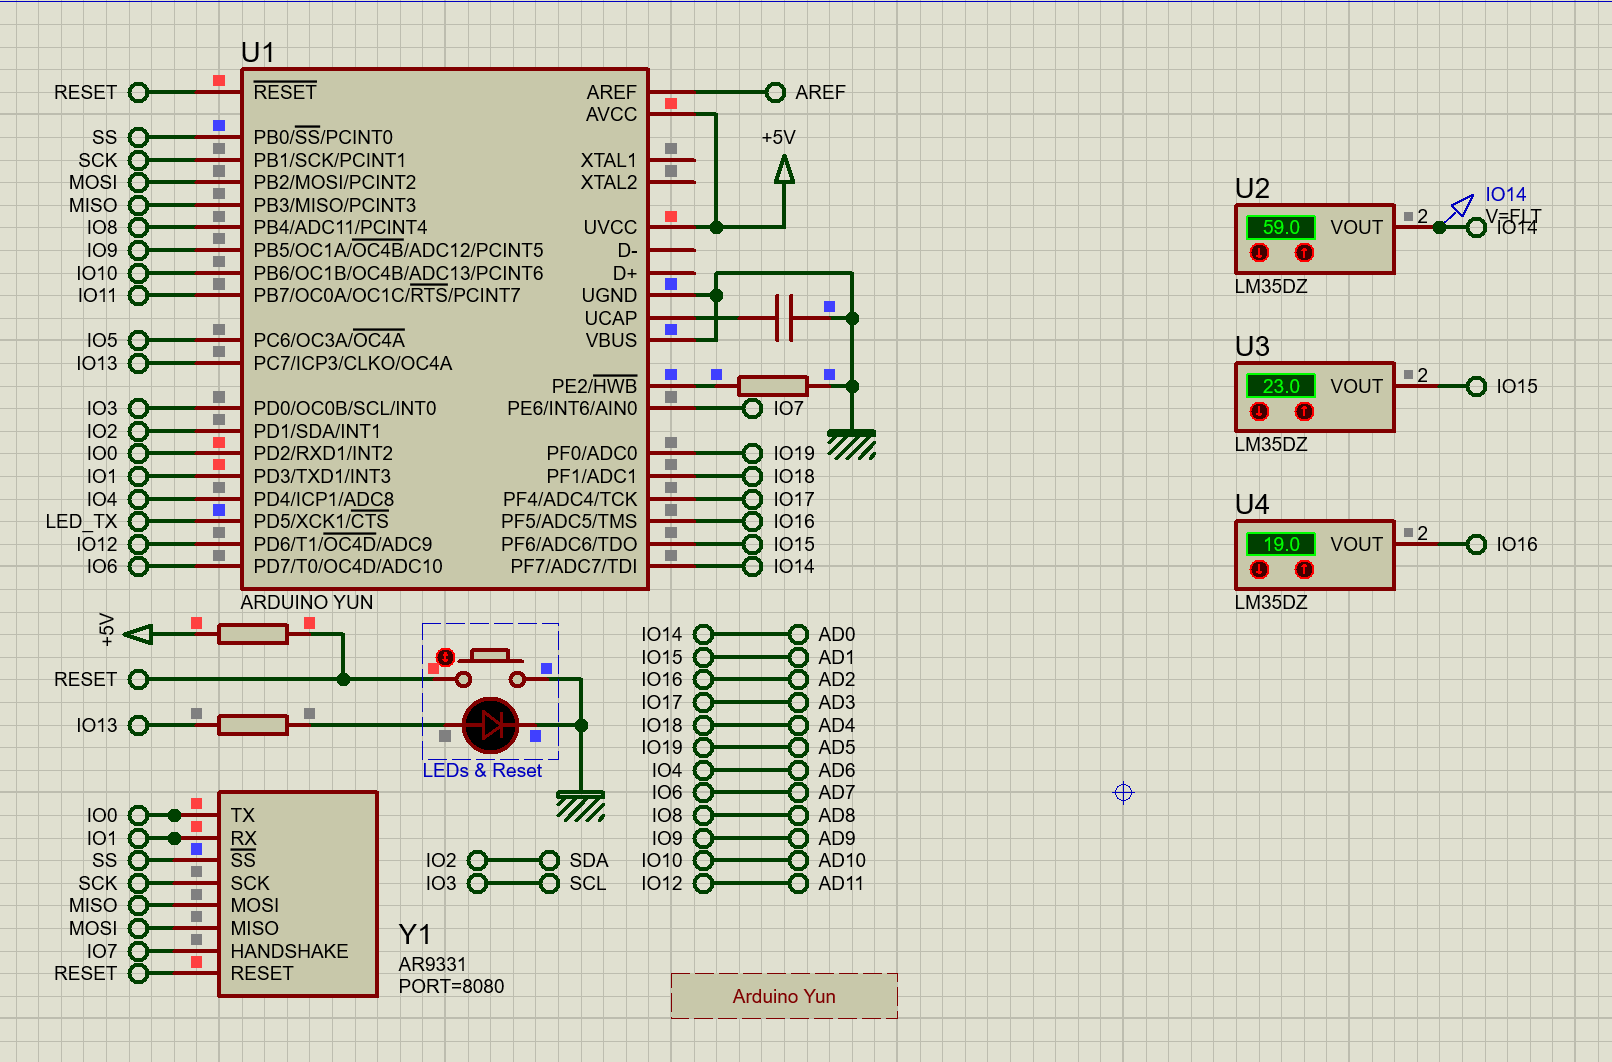
\includegraphics[width=\linewidth]{figs/circuit.png}
	\caption{شماتیک مدار}
\end{figure}

\subsection{توضیح کلی کد}
اینجا کلا توضیج میدیم که کد چه جوریه و سیستم چه جوریه و اینا

\subsection{اپلیکیشن گوشی}
برای طراحی اپلیکیشن گوشی ما از قابلیت‌های 
\lr{Visual Designer}
استفاده کردیم و کنترلر‌های 
\lr{iot}
زیر را 

- عکس از پنل گوشی

- توضیج این که چطوری از طریق وای فای با اضافه کردن ip دستگاه از روی گوشی ریزالتو می بینیم و اینا

\subsection{وب‌سرور و میانگین‌گیری از نتایج چند دستگاه}
- اینجا راجع به  
elastic search
 اینا توضیح میدیم و ساختن ایندکسو پوش کردن ریزالتا و ...

\section{فایل‌ها و شیوه ‌ی اجرای برنامه}
- اینجا یه توضیحی میدیم که کلا فایلا چین و کی کجاست و ران گرفتن چه جوریه. من یه سری فایل برای الستیک هم گذاشتم برای ساخت ایندکس و اینا. 

\section{سیمولیشن و نتایج}
- یه تعدادی عکس از اجرای برنامه از روی گوشی با یه لوکیشن و از روی وب سرور با مثلا دو تا لوکیشن


